\section{$\mathbf{t}$-Probability Table}
\label{tDistributionTable}

A \term{t-probability table} may be used to
find tail areas of a $t$-distribution using a T-score,
or vice-versa.
Such a table lists T-scores and the corresponding percentiles.
A partial \term{t-table} is shown in Figure~\ref{tTableSample},
and the complete table starts on page~\pageref{tTableFirstPage}.
Each row in the $t$-table represents a $t$-distribution with
different degrees of freedom.
The columns correspond to tail probabilities.
For instance, if we know we are working with the
$t$-distribution with $df=18$, we can examine row 18,
which is highlighted in Figure~\ref{tTableSample}.
If we want the value in this row that identifies the T-score
(cutoff) for an upper tail of 10\%, we can look in the column
where \emph{one tail} is 0.100.
This cutoff is 1.33.
If we had wanted the cutoff for the lower 10\%, we would
use -1.33.
Just like the normal distribution,
all $t$-distributions are symmetric.

\begin{figure}[hht]
\centering
\begin{tabular}{r | rrr rr}
one tail & \hspace{1.5mm}  0.100 & \hspace{1.5mm} 0.050 & \hspace{1.5mm} 0.025 & \hspace{1.5mm} 0.010 & \hspace{1.5mm} 0.005  \\
two tails & 0.200 & 0.100 & 0.050 & 0.020 & 0.010 \\
\hline
{$df$} \hfill 1  &  {\normalsize  3.08} & {\normalsize  6.31} & {\normalsize 12.71} & {\normalsize 31.82} & {\normalsize 63.66}  \\ 
2  &  {\normalsize  1.89} & {\normalsize  2.92} & {\normalsize  4.30} & {\normalsize  6.96} & {\normalsize  9.92}  \\ 
3  &  {\normalsize  1.64} & {\normalsize  2.35} & {\normalsize  3.18} & {\normalsize  4.54} & {\normalsize  5.84}  \\ 
$\vdots$ & $\vdots$ &$\vdots$ &$\vdots$ &$\vdots$ & \\
17  &  {\normalsize  1.33} & {\normalsize  1.74} & {\normalsize  2.11} & {\normalsize  2.57} & {\normalsize  2.90}  \\ 
\highlightO{18}  &  \highlightO{\normalsize  1.33} & \highlightO{\normalsize  1.73} & \highlightO{\normalsize  2.10} & \highlightO{\normalsize  2.55} & \highlightO{\normalsize  2.88}  \\ 
19  &  {\normalsize  1.33} & {\normalsize  1.73} & {\normalsize  2.09} & {\normalsize  2.54} & {\normalsize  2.86}  \\ 
20  &  {\normalsize  1.33} & {\normalsize  1.72} & {\normalsize  2.09} & {\normalsize  2.53} & {\normalsize  2.85}  \\ 
$\vdots$ & $\vdots$ &$\vdots$ &$\vdots$ &$\vdots$ & \\
400  &  {\normalsize  1.28} & {\normalsize  1.65} & {\normalsize  1.97} & {\normalsize  2.34} & {\normalsize  2.59}  \\ 
500  &  {\normalsize  1.28} & {\normalsize  1.65} & {\normalsize  1.96} & {\normalsize  2.33} & {\normalsize  2.59}  \\ 
$\infty$  &  {\normalsize  1.28} & {\normalsize  1.64} & {\normalsize  1.96} & {\normalsize  2.33} & {\normalsize  2.58}  \\ 
\end{tabular}
\caption{An abbreviated look at the $t$-table.
    Each row represents a different $t$-distribution.
    The columns describe the cutoffs for specific tail areas.
    The row with $df=18$ has been \highlightO{highlighted}.}
\label{tTableSample}
\end{figure}

\begin{examplewrap}
\begin{nexample}{What proportion of the $t$-distribution with
    18 degrees of freedom falls below -2.10?}
  Just like a normal probability problem, we first draw the
  picture and shade the area below -2.10:
  \begin{center}
  \includegraphics[width=0.5\textwidth]{ch_inference_for_means/figures/tDistDF18LeftTail2Point10/tDistDF18LeftTail2Point10}
  \end{center}
  To find this area, we first identify the appropriate row:
  $df = 18$.
  Then we identify the column containing the absolute value
  of -2.10;
  it~is the third column.
  Because we are looking for just one tail, we examine the
  top line of the table, which shows that a one tail area
  for a value in the third row corresponds to 0.025.
  That is, 2.5\% of the distribution falls below -2.10.

  In the next example we encounter a case where the exact
  T-score is not listed in the table.
\end{nexample}
\end{examplewrap}

\begin{examplewrap}
\begin{nexample}{A $t$-distribution with 20 degrees of freedom
    is shown in the left panel of
    Figure~\ref{tDistAppendixTwoEx}.
    Estimate the proportion of the distribution falling
    above~1.65.}
  We identify the row in the $t$-table using the degrees
  of freedom: $df=20$.
  Then we look for 1.65; it is not listed.
  It falls between the first and second columns.
  Since these values bound 1.65, their tail areas will
  bound the tail area corresponding to 1.65.
  We identify the one tail area of the first and
  second columns, 0.050 and 0.10, and we conclude that
  between 5\% and 10\% of the distribution is more than
  1.65 standard deviations above the mean.
  If we like, we can identify the precise area using
  statistical software: 0.0573.
\end{nexample}
\end{examplewrap}

\begin{figure}[h]
\centering
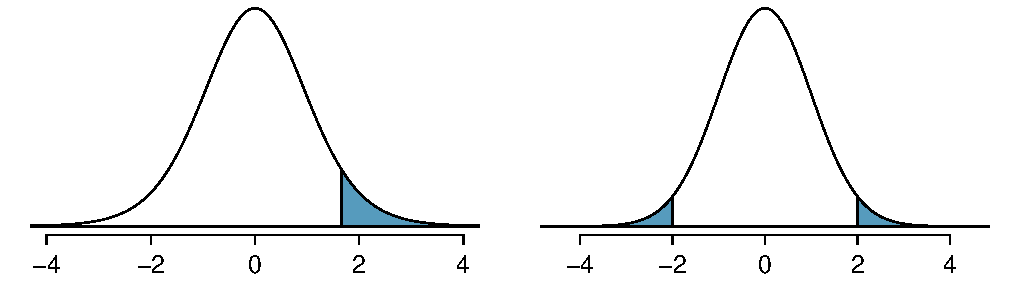
\includegraphics[width=0.85\textwidth]{ch_inference_for_means/figures/tDistAppendixTwoEx/tDistAppendixTwoEx}
\caption{Left: The $t$-distribution with 20 degrees of freedom,
    with the area above 1.65 shaded.
    Right: The $t$-distribution with 475 degrees of freedom,
    with the area further than 2 units from 0 shaded.}
\label{tDistAppendixTwoEx}
\end{figure}

\begin{examplewrap}
\begin{nexample}{A $t$-distribution with 475 degrees of freedom
    is shown in the right panel of
    Figure~\ref{tDistAppendixTwoEx}.
    Estimate the proportion of the distribution falling more
    than 2 units from the mean (above or below).}
  As before, first identify the appropriate row: $df=475$.
  This row does not exist!
  When this happens, we use the next smaller row, which in
  this case is $df = 400$.
  Next, find the columns that capture 2.00;
  because $1.97 < 3 < 2.34$, we use the third and fourth columns.
  Finally, we find bounds for the tail areas by looking at
  the two tail values: 0.02 and 0.05.
  We use the two tail values because we are looking for two
  symmetric tails in the $t$-distribution.
\end{nexample}
\end{examplewrap}

\begin{exercisewrap}
\begin{nexercise}
What proportion of the $t$-distribution with 19 degrees of freedom falls above -1.79 units?\footnotemark{}
\end{nexercise}
\end{exercisewrap}
\footnotetext{We find the shaded area \emph{above} -1.79 (we leave the picture to you). The small left tail is between 0.025 and 0.05, so the larger upper region must have an area between 0.95 and 0.975.}

\begin{examplewrap}
\begin{nexample}{Find the value of $t_{18}^{\star}$
    using the $t$-table, where $t_{18}^{\star}$
    is the cutoff for the $t$-distribution with
    18 degrees of freedom where 95\% of the distribution
    lies between -$t_{18}^{\star}$ and +$t_{18}^{\star}$.}
  For a 95\% confidence interval, we want to find
  the cutoff $t^{\star}_{18}$ such that 95\% of the
  $t$-distribution is between -$t^{\star}_{18}$
  and $t^{\star}_{18}$;
  this is the same as where the two tails have a total
  area of 0.05.
  We look in the $t$-table on page~\pageref{tTableSample},
  find the column with area totaling 0.05 in the two tails
  (third column), and then the row with 18 degrees of
  freedom: $t^{\star}_{18} = 2.10$.
\end{nexample}
\end{examplewrap}


\newpage

\begin{center}
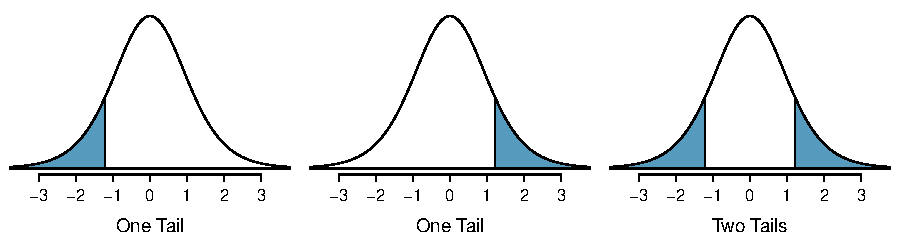
\includegraphics[width=\textwidth]
    {extraTeX/tables/figures/tTails/tTails}
\end{center}

\begin{center}
\begin{tabular}{r | rrr rr}
\hline
one tail & \hspace{1.5mm}  0.100 & \hspace{1.5mm} 0.050 & \hspace{1.5mm} 0.025 & \hspace{1.5mm} 0.010 & \hspace{1.5mm} 0.005  \\
two tails & 0.200 & 0.100 & 0.050 & 0.020 & 0.010 \\
\hline
{df} \hfill 1  &  {\normalsize  3.08} & {\normalsize  6.31} & {\normalsize 12.71} & {\normalsize 31.82} & {\normalsize 63.66}  \\ 
2  &  {\normalsize  1.89} & {\normalsize  2.92} & {\normalsize  4.30} & {\normalsize  6.96} & {\normalsize  9.92}  \\ 
3  &  {\normalsize  1.64} & {\normalsize  2.35} & {\normalsize  3.18} & {\normalsize  4.54} & {\normalsize  5.84}  \\ 
4  &  {\normalsize  1.53} & {\normalsize  2.13} & {\normalsize  2.78} & {\normalsize  3.75} & {\normalsize  4.60}  \\ 
5  &  {\normalsize  1.48} & {\normalsize  2.02} & {\normalsize  2.57} & {\normalsize  3.36} & {\normalsize  4.03}  \\ 
\hline
6  &  {\normalsize  1.44} & {\normalsize  1.94} & {\normalsize  2.45} & {\normalsize  3.14} & {\normalsize  3.71}  \\ 
7  &  {\normalsize  1.41} & {\normalsize  1.89} & {\normalsize  2.36} & {\normalsize  3.00} & {\normalsize  3.50}  \\ 
8  &  {\normalsize  1.40} & {\normalsize  1.86} & {\normalsize  2.31} & {\normalsize  2.90} & {\normalsize  3.36}  \\ 
9  &  {\normalsize  1.38} & {\normalsize  1.83} & {\normalsize  2.26} & {\normalsize  2.82} & {\normalsize  3.25}  \\ 
10  &  {\normalsize  1.37} & {\normalsize  1.81} & {\normalsize  2.23} & {\normalsize  2.76} & {\normalsize  3.17}  \\ 
\hline
\hline
11  &  {\normalsize  1.36} & {\normalsize  1.80} & {\normalsize  2.20} & {\normalsize  2.72} & {\normalsize  3.11}  \\ 
12  &  {\normalsize  1.36} & {\normalsize  1.78} & {\normalsize  2.18} & {\normalsize  2.68} & {\normalsize  3.05}  \\ 
13  &  {\normalsize  1.35} & {\normalsize  1.77} & {\normalsize  2.16} & {\normalsize  2.65} & {\normalsize  3.01}  \\ 
14  &  {\normalsize  1.35} & {\normalsize  1.76} & {\normalsize  2.14} & {\normalsize  2.62} & {\normalsize  2.98}  \\ 
15  &  {\normalsize  1.34} & {\normalsize  1.75} & {\normalsize  2.13} & {\normalsize  2.60} & {\normalsize  2.95}  \\ 
\hline
16  &  {\normalsize  1.34} & {\normalsize  1.75} & {\normalsize  2.12} & {\normalsize  2.58} & {\normalsize  2.92}  \\ 
17  &  {\normalsize  1.33} & {\normalsize  1.74} & {\normalsize  2.11} & {\normalsize  2.57} & {\normalsize  2.90}  \\ 
18  &  {\normalsize  1.33} & {\normalsize  1.73} & {\normalsize  2.10} & {\normalsize  2.55} & {\normalsize  2.88}  \\ 
19  &  {\normalsize  1.33} & {\normalsize  1.73} & {\normalsize  2.09} & {\normalsize  2.54} & {\normalsize  2.86}  \\ 
20  &  {\normalsize  1.33} & {\normalsize  1.72} & {\normalsize  2.09} & {\normalsize  2.53} & {\normalsize  2.85}  \\ 
\hline
\hline
21  &  {\normalsize  1.32} & {\normalsize  1.72} & {\normalsize  2.08} & {\normalsize  2.52} & {\normalsize  2.83}  \\ 
22  &  {\normalsize  1.32} & {\normalsize  1.72} & {\normalsize  2.07} & {\normalsize  2.51} & {\normalsize  2.82}  \\ 
23  &  {\normalsize  1.32} & {\normalsize  1.71} & {\normalsize  2.07} & {\normalsize  2.50} & {\normalsize  2.81}  \\ 
24  &  {\normalsize  1.32} & {\normalsize  1.71} & {\normalsize  2.06} & {\normalsize  2.49} & {\normalsize  2.80}  \\ 
25  &  {\normalsize  1.32} & {\normalsize  1.71} & {\normalsize  2.06} & {\normalsize  2.49} & {\normalsize  2.79}  \\ 
\hline
26  &  {\normalsize  1.31} & {\normalsize  1.71} & {\normalsize  2.06} & {\normalsize  2.48} & {\normalsize  2.78}  \\ 
27  &  {\normalsize  1.31} & {\normalsize  1.70} & {\normalsize  2.05} & {\normalsize  2.47} & {\normalsize  2.77}  \\ 
28  &  {\normalsize  1.31} & {\normalsize  1.70} & {\normalsize  2.05} & {\normalsize  2.47} & {\normalsize  2.76}  \\ 
29  &  {\normalsize  1.31} & {\normalsize  1.70} & {\normalsize  2.05} & {\normalsize  2.46} & {\normalsize  2.76}  \\ 
30  &  {\normalsize  1.31} & {\normalsize  1.70} & {\normalsize  2.04} & {\normalsize  2.46} & {\normalsize  2.75}  \\ 
\hline
\end{tabular}
\label{tTableFirstPage}
\end{center}


\newpage

\begin{center}
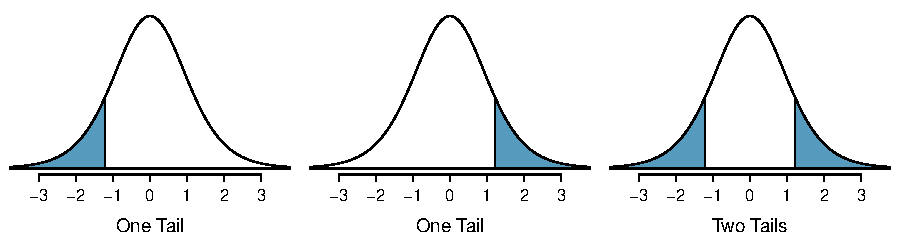
\includegraphics[width=\textwidth]
    {extraTeX/tables/figures/tTails/tTails}
\end{center}

\begin{center}
\begin{tabular}{r | rrr rr}
\hline
one tail & \hspace{1.5mm}  0.100 & \hspace{1.5mm} 0.050 & \hspace{1.5mm} 0.025 & \hspace{1.5mm} 0.010 & \hspace{1.5mm} 0.005  \\
two tails & 0.200 & 0.100 & 0.050 & 0.020 & 0.010 \\
\hline
{df} \hfill 31  &  {\normalsize  1.31} & {\normalsize  1.70} & {\normalsize  2.04} & {\normalsize  2.45} & {\normalsize  2.74}  \\ 
32  &  {\normalsize  1.31} & {\normalsize  1.69} & {\normalsize  2.04} & {\normalsize  2.45} & {\normalsize  2.74}  \\ 
33  &  {\normalsize  1.31} & {\normalsize  1.69} & {\normalsize  2.03} & {\normalsize  2.44} & {\normalsize  2.73}  \\ 
34  &  {\normalsize  1.31} & {\normalsize  1.69} & {\normalsize  2.03} & {\normalsize  2.44} & {\normalsize  2.73}  \\ 
35  &  {\normalsize  1.31} & {\normalsize  1.69} & {\normalsize  2.03} & {\normalsize  2.44} & {\normalsize  2.72}  \\ 
\hline
36  &  {\normalsize  1.31} & {\normalsize  1.69} & {\normalsize  2.03} & {\normalsize  2.43} & {\normalsize  2.72}  \\ 
37  &  {\normalsize  1.30} & {\normalsize  1.69} & {\normalsize  2.03} & {\normalsize  2.43} & {\normalsize  2.72}  \\ 
38  &  {\normalsize  1.30} & {\normalsize  1.69} & {\normalsize  2.02} & {\normalsize  2.43} & {\normalsize  2.71}  \\ 
39  &  {\normalsize  1.30} & {\normalsize  1.68} & {\normalsize  2.02} & {\normalsize  2.43} & {\normalsize  2.71}  \\ 
40  &  {\normalsize  1.30} & {\normalsize  1.68} & {\normalsize  2.02} & {\normalsize  2.42} & {\normalsize  2.70}  \\ 
\hline
\hline
41  &  {\normalsize  1.30} & {\normalsize  1.68} & {\normalsize  2.02} & {\normalsize  2.42} & {\normalsize  2.70}  \\ 
42  &  {\normalsize  1.30} & {\normalsize  1.68} & {\normalsize  2.02} & {\normalsize  2.42} & {\normalsize  2.70}  \\ 
43  &  {\normalsize  1.30} & {\normalsize  1.68} & {\normalsize  2.02} & {\normalsize  2.42} & {\normalsize  2.70}  \\ 
44  &  {\normalsize  1.30} & {\normalsize  1.68} & {\normalsize  2.02} & {\normalsize  2.41} & {\normalsize  2.69}  \\ 
45  &  {\normalsize  1.30} & {\normalsize  1.68} & {\normalsize  2.01} & {\normalsize  2.41} & {\normalsize  2.69}  \\ 
\hline
46  &  {\normalsize  1.30} & {\normalsize  1.68} & {\normalsize  2.01} & {\normalsize  2.41} & {\normalsize  2.69}  \\ 
47  &  {\normalsize  1.30} & {\normalsize  1.68} & {\normalsize  2.01} & {\normalsize  2.41} & {\normalsize  2.68}  \\ 
48  &  {\normalsize  1.30} & {\normalsize  1.68} & {\normalsize  2.01} & {\normalsize  2.41} & {\normalsize  2.68}  \\ 
49  &  {\normalsize  1.30} & {\normalsize  1.68} & {\normalsize  2.01} & {\normalsize  2.40} & {\normalsize  2.68}  \\ 
50  &  {\normalsize  1.30} & {\normalsize  1.68} & {\normalsize  2.01} & {\normalsize  2.40} & {\normalsize  2.68}  \\ 
\hline
\hline
%55  &  {\normalsize  1.30} & {\normalsize  1.67} & {\normalsize  2.00} & {\normalsize  2.40} & {\normalsize  2.67}  \\ 
60  &  {\normalsize  1.30} & {\normalsize  1.67} & {\normalsize  2.00} & {\normalsize  2.39} & {\normalsize  2.66}  \\ 
%65  &  {\normalsize  1.29} & {\normalsize  1.67} & {\normalsize  2.00} & {\normalsize  2.39} & {\normalsize  2.65}  \\ 
70  &  {\normalsize  1.29} & {\normalsize  1.67} & {\normalsize  1.99} & {\normalsize  2.38} & {\normalsize  2.65}  \\ 
%75  &  {\normalsize  1.29} & {\normalsize  1.67} & {\normalsize  1.99} & {\normalsize  2.38} & {\normalsize  2.64}  \\ 
%\hline
80  &  {\normalsize  1.29} & {\normalsize  1.66} & {\normalsize  1.99} & {\normalsize  2.37} & {\normalsize  2.64}  \\ 
%85  &  {\normalsize  1.29} & {\normalsize  1.66} & {\normalsize  1.99} & {\normalsize  2.37} & {\normalsize  2.63}  \\ 
90  &  {\normalsize  1.29} & {\normalsize  1.66} & {\normalsize  1.99} & {\normalsize  2.37} & {\normalsize  2.63}  \\ 
%95  &  {\normalsize  1.29} & {\normalsize  1.66} & {\normalsize  1.99} & {\normalsize  2.37} & {\normalsize  2.63}  \\ 
100  &  {\normalsize  1.29} & {\normalsize  1.66} & {\normalsize  1.98} & {\normalsize  2.36} & {\normalsize  2.63}  \\ 
\hline
%\hline
%120  &  {\normalsize  1.29} & {\normalsize  1.66} & {\normalsize  1.98} & {\normalsize  2.36} & {\normalsize  2.62}  \\ 
%140  &  {\normalsize  1.29} & {\normalsize  1.66} & {\normalsize  1.98} & {\normalsize  2.35} & {\normalsize  2.61}  \\ 
150  &  {\normalsize  1.29} & {\normalsize  1.66} & {\normalsize  1.98} & {\normalsize  2.35} & {\normalsize  2.61}  \\ 
%160  &  {\normalsize  1.29} & {\normalsize  1.65} & {\normalsize  1.97} & {\normalsize  2.35} & {\normalsize  2.61}  \\ 
%180  &  {\normalsize  1.29} & {\normalsize  1.65} & {\normalsize  1.97} & {\normalsize  2.35} & {\normalsize  2.60}  \\ 
200  &  {\normalsize  1.29} & {\normalsize  1.65} & {\normalsize  1.97} & {\normalsize  2.35} & {\normalsize  2.60}  \\ 
%\hline
300  &  {\normalsize  1.28} & {\normalsize  1.65} & {\normalsize  1.97} & {\normalsize  2.34} & {\normalsize  2.59}  \\ 
400  &  {\normalsize  1.28} & {\normalsize  1.65} & {\normalsize  1.97} & {\normalsize  2.34} & {\normalsize  2.59}  \\ 
500  &  {\normalsize  1.28} & {\normalsize  1.65} & {\normalsize  1.96} & {\normalsize  2.33} & {\normalsize  2.59}  \\ 
\hline
\hline
$\infty$  &  {\normalsize  1.28} & {\normalsize  1.65} & {\normalsize  1.96} & {\normalsize  2.33} & {\normalsize  2.58}  \\ 
\hline
\end{tabular}
\end{center}

